\documentclass[aspectratio=169]{beamer}
\usepackage{lmodern}
%\usetheme{Madrid}
%\usecolortheme{giantoak}
\newcommand*\oldmacro{}
\let\oldmacro\insertshorttitle
\renewcommand*\insertshorttitle{\oldmacro\hfill\insertframenumber\,/\,\inserttotalframenumber}
\usepackage[framemethod=tikz]{mdframed}

%\usepackage{beamerthemesplit}
\usepackage{textpos}
\usepackage{pgf}
\usepackage{ulem}
%\logo{\pgfputat{\pgfxy(0,-.4)}{\pgfbox[right,base]{\includegraphics[height=1.0cm]{logo.jpg}}}}
%\newcommand{\nologo}{\setbeamertemplate{logo}{}}
\usepackage{booktabs}
\usepackage{graphicx}
\theoremstyle{principle}
\newtheorem*{principle}{Design Principle}


\titlegraphic{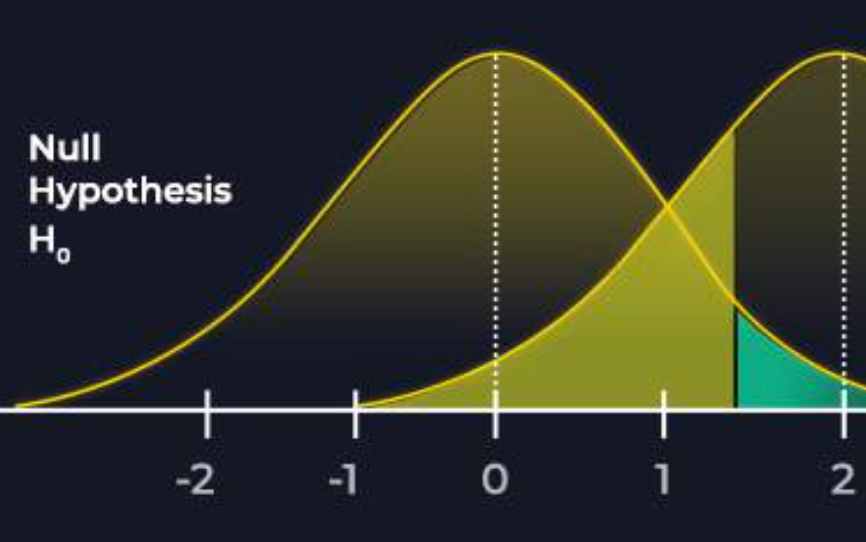
\includegraphics[width=1.0\paperwidth]{distros.png}}

\title{Amendments}
%\author[Jeremy Kedziora]{Wind Data Science Team\\
%\small{Uptake}}
\date{}

\begin{document}

%{
%%\nologo
%\begin{frame}
%    \maketitle
%\end{frame}
%}
%pages 1-7, 8-9, 14-15.


{
%  \usebackgroundtemplate{
\includegraphics[width=1.0\paperwidth]{statistics-review.jpg}}
  \usebackgroundtemplate{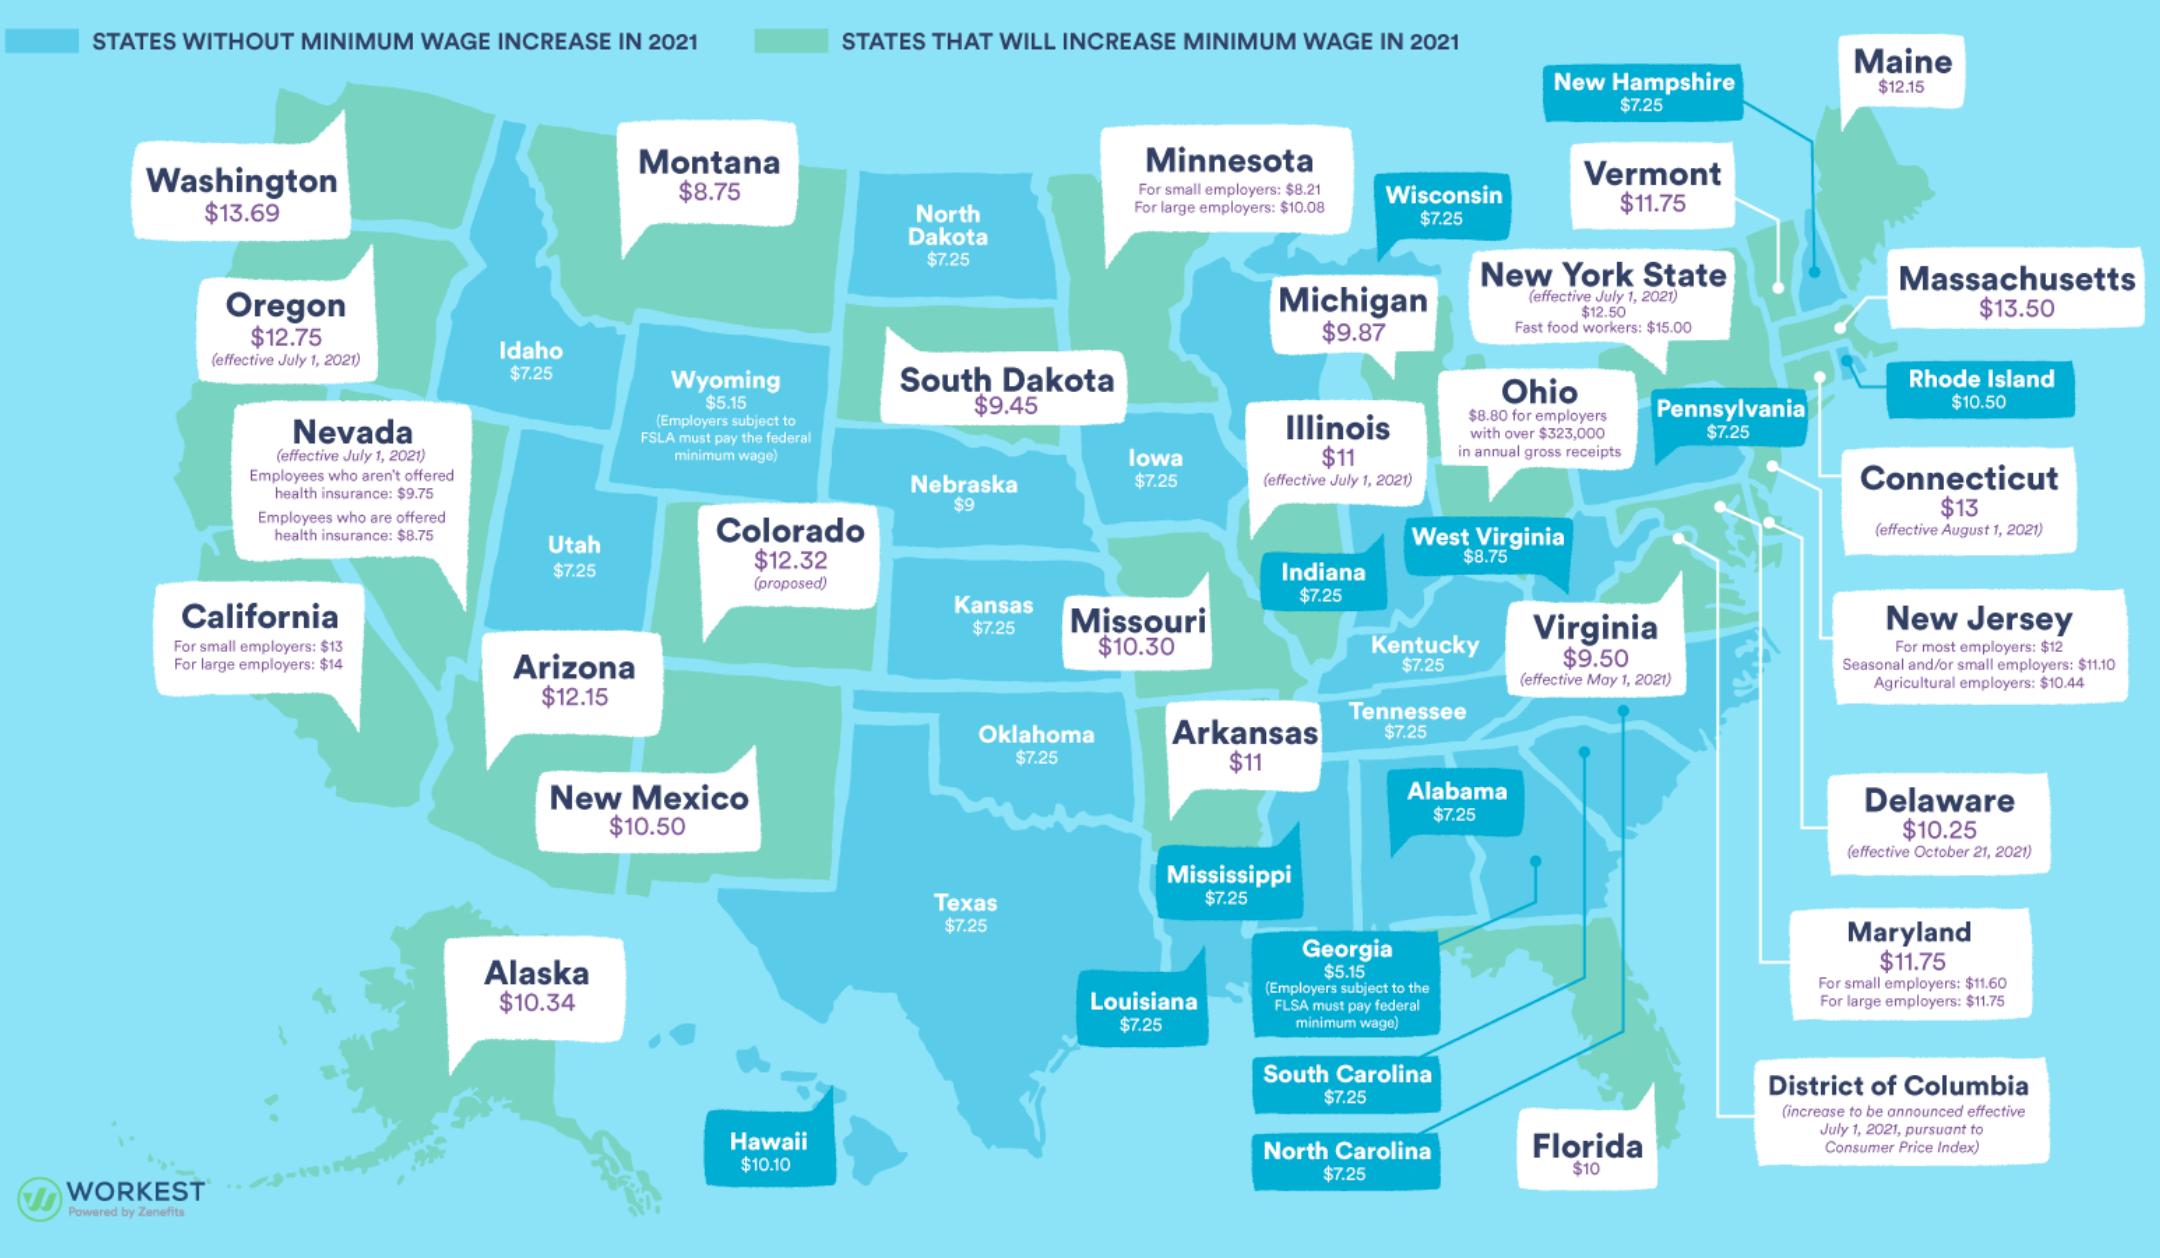
\includegraphics[scale=0.42]{min_wage.png}}
  \begin{frame}[plain]
  
\begin{mdframed}[tikzsetting={draw=white,fill=white,fill opacity=0.6,draw opacity=0.4,
               line width=0pt},backgroundcolor=none,leftmargin=20,
               rightmargin=20,innertopmargin=4pt]
\begin{center}
\Huge \textbf{Difference in Differences}
\end{center}
\end{mdframed}

  \end{frame}
}

%most reliant on human cognition
%limited only by cognition
%hypothesis generating scheme often functioning as a gateway into more statistical analysis

%%@@@@@@@@@@@@@@@@@@@@@@@@@@@@@@@@@@@@@@@@@@@@@@@@@
%\begin{frame}
%\frametitle{Napoleon's Progress}
%\begin{center}
%
\includegraphics[scale=0.4]{experiment.png}
%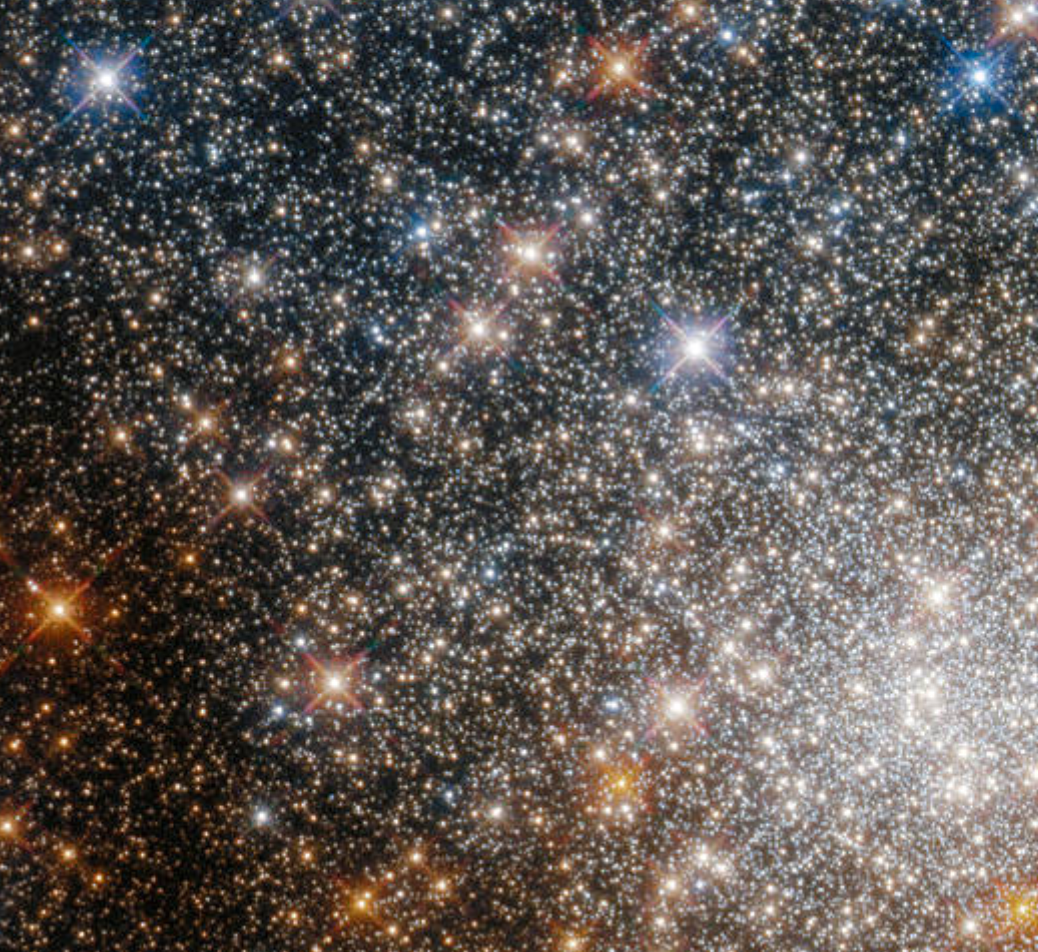
\includegraphics[scale=0.35]{stars.png}
%\end{center}
%
%\end{frame}

%@@@@@@@@@@@@@@@@@@@@@@@@@@@@@@@@@@@@@@@@@@@@@@@@@
\begin{frame}
\frametitle{Today:}

\begin{itemize}
\item Extend linear regression to make the most of natural experiment type data;
\bigskip
\bigskip
\bigskip

\item Work through a case study applying difference in differences.

\end{itemize}

\end{frame}

%@@@@@@@@@@@@@@@@@@@@@@@@@@@@@@@@@@@@@@@@@@@@@@@@@
\begin{frame}
\frametitle{So far, we've used linear regression to:}

\begin{enumerate} 
\item Model a linear relationship between dependent variable $y$ and independent variable $x$:
\begin{align*}
y = \beta_0 + \beta_1x + \varepsilon;
\end{align*}

\item Model a linear relationship between dependent variable $y$ and many independent variables $x_1,x_2,x_3,\hdots$:
\begin{align*}
y = \beta_0 + \beta_1x_1 + \beta_2x_2 + \beta_3x_3 + \hdots + \varepsilon;
\end{align*}

\item Model a NON-linear relationship between dependent variable $y$ and many independent variables $x$:
\begin{align*}
y = \beta_0 + \beta_1x_1 + \beta_2x_1^2 + \hdots + \varepsilon;
\end{align*}

\item Model relationships between independent variables:
\begin{align*}
y = \beta_0 + \beta_1x_1 + \beta_2x_2 + \beta_{12}x_1x_2 + \varepsilon;
\end{align*}

\end{enumerate}

\end{frame}

%@@@@@@@@@@@@@@@@@@@@@@@@@@@@@@@@@@@@@@@@@@@@@@@@@
\begin{frame}
\frametitle{Motivation...}

\begin{center}
\Huge\textbf{Does increasing the minimum wage decrease employment?}\\
\end{center}

\end{frame}

%@@@@@@@@@@@@@@@@@@@@@@@@@@@@@@@@@@@@@@@@@@@@@@@@@
\begin{frame}
\frametitle{Motivation...}


\begin{columns}
\begin{column}{0.5\textwidth}

\begin{itemize}

\item In early 1990 NJ raised the minimum wage from \$4.25 to \$5.05 effective 1 April 1992 -- highest minimum wage in the country;
\bigskip

\item Notably, nearby eastern PA maintained a lower minimum wage;
\bigskip

\item A \textbf{natural} within-subjects experiment;
\begin{itemize}
\item NJ employers before/after;
\item PA employers before/after;
\end{itemize}
\bigskip

\item Card and Krueger surveyed 473 fast food restaurants before and after law;
\begin{itemize}
\item Low wage workers;
\item High response survey response rate.
\end{itemize}

\end{itemize}

\end{column}
\begin{column}{0.5\textwidth}
\begin{center}
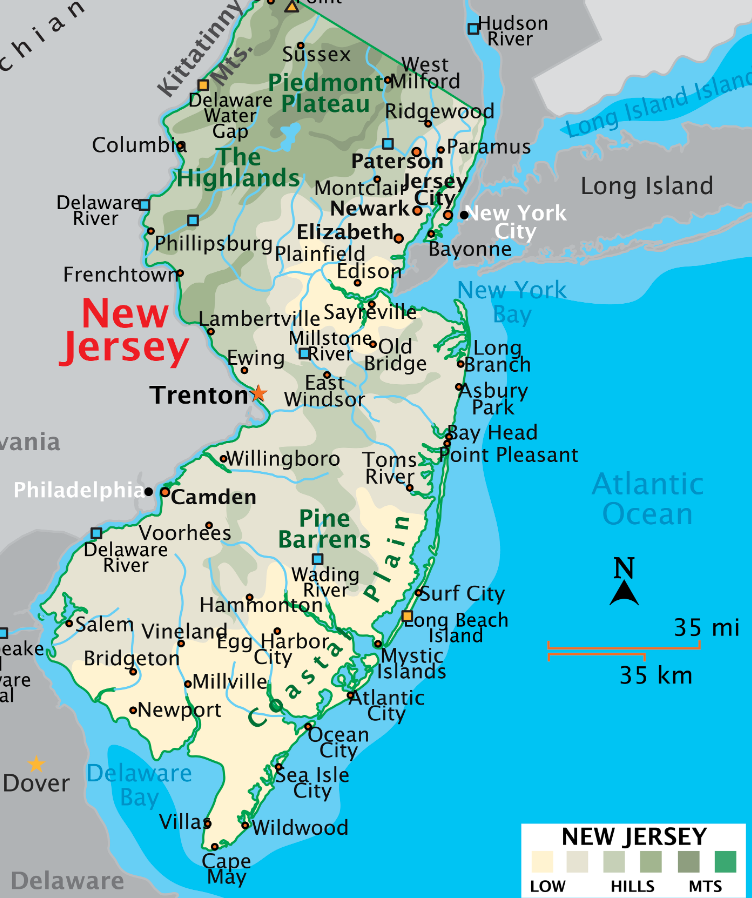
\includegraphics[scale=0.4]{nj_map.png}
\end{center}
\end{column}
\end{columns}

\end{frame}

%@@@@@@@@@@@@@@@@@@@@@@@@@@@@@@@@@@@@@@@@@@@@@@@@@
\begin{frame}

\begin{center}
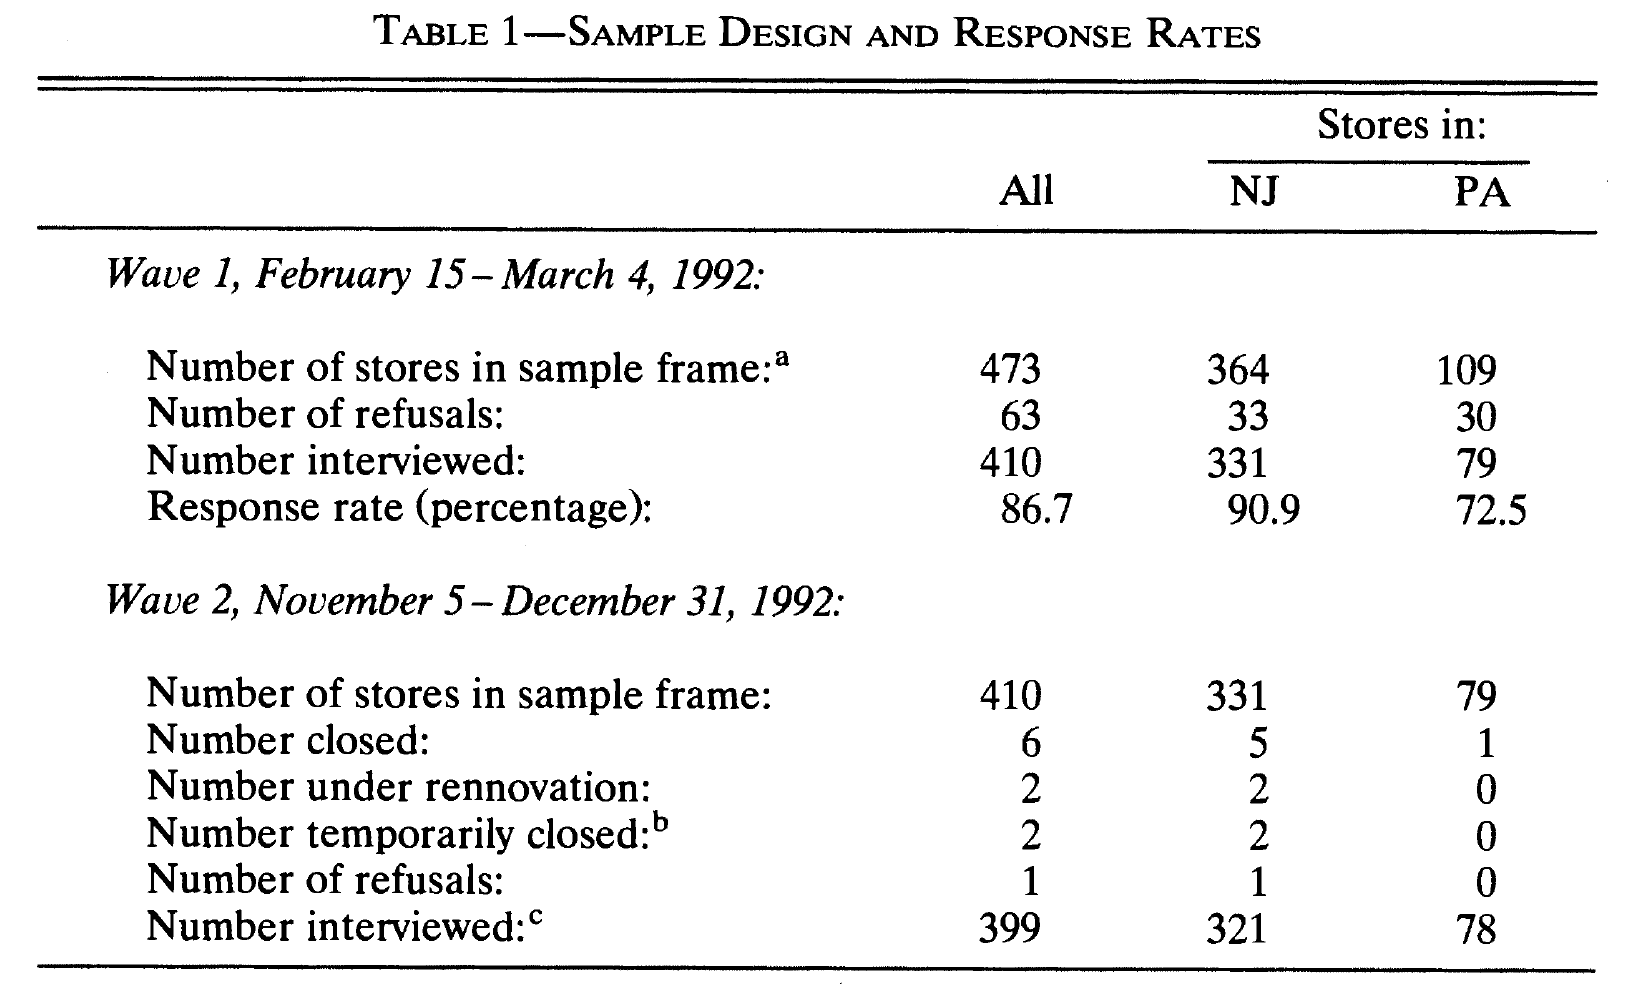
\includegraphics[scale=0.4]{response_rates.png}
\end{center}

\end{frame}

%@@@@@@@@@@@@@@@@@@@@@@@@@@@@@@@@@@@@@@@@@@@@@@@@@
\begin{frame}

\begin{center}
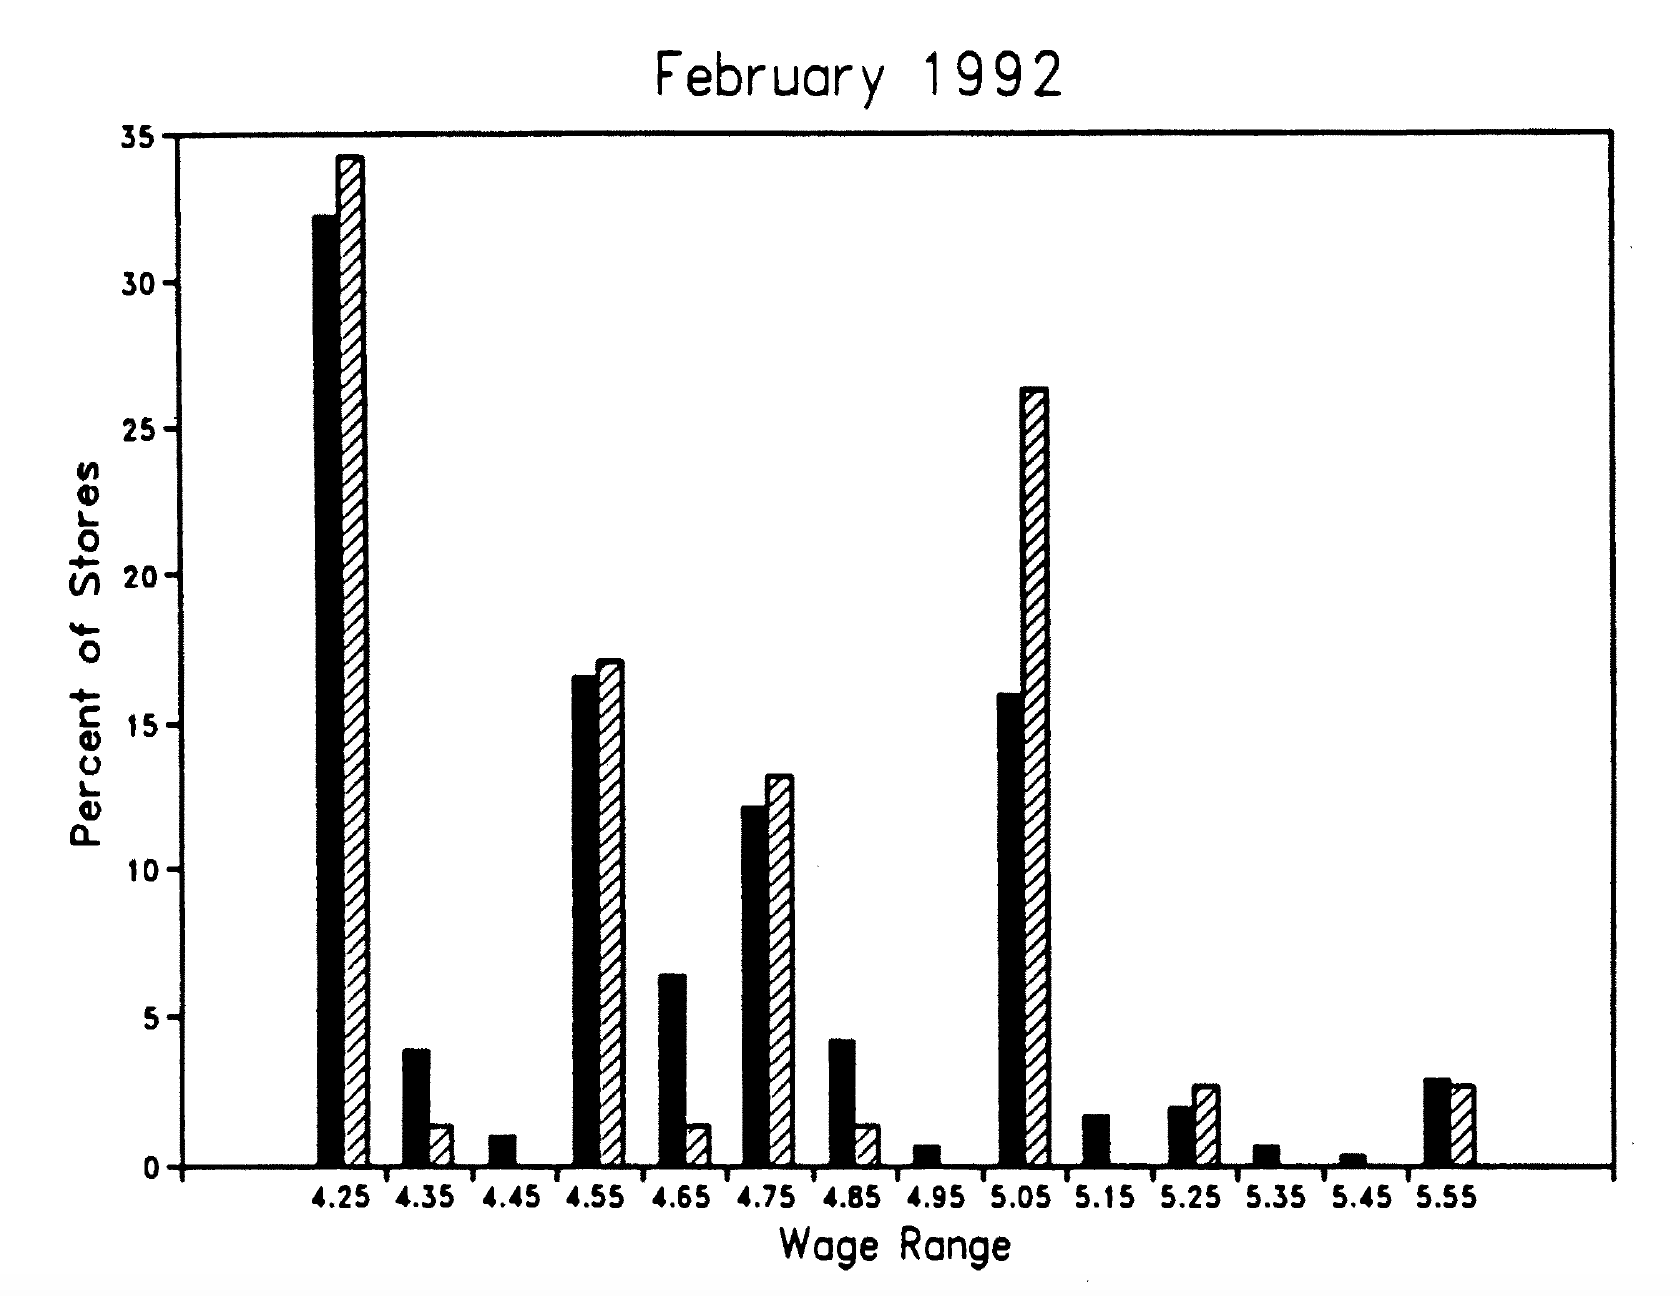
\includegraphics[scale=0.35]{feb_1992.png}
\end{center}

\end{frame}

%@@@@@@@@@@@@@@@@@@@@@@@@@@@@@@@@@@@@@@@@@@@@@@@@@
\begin{frame}

\begin{center}
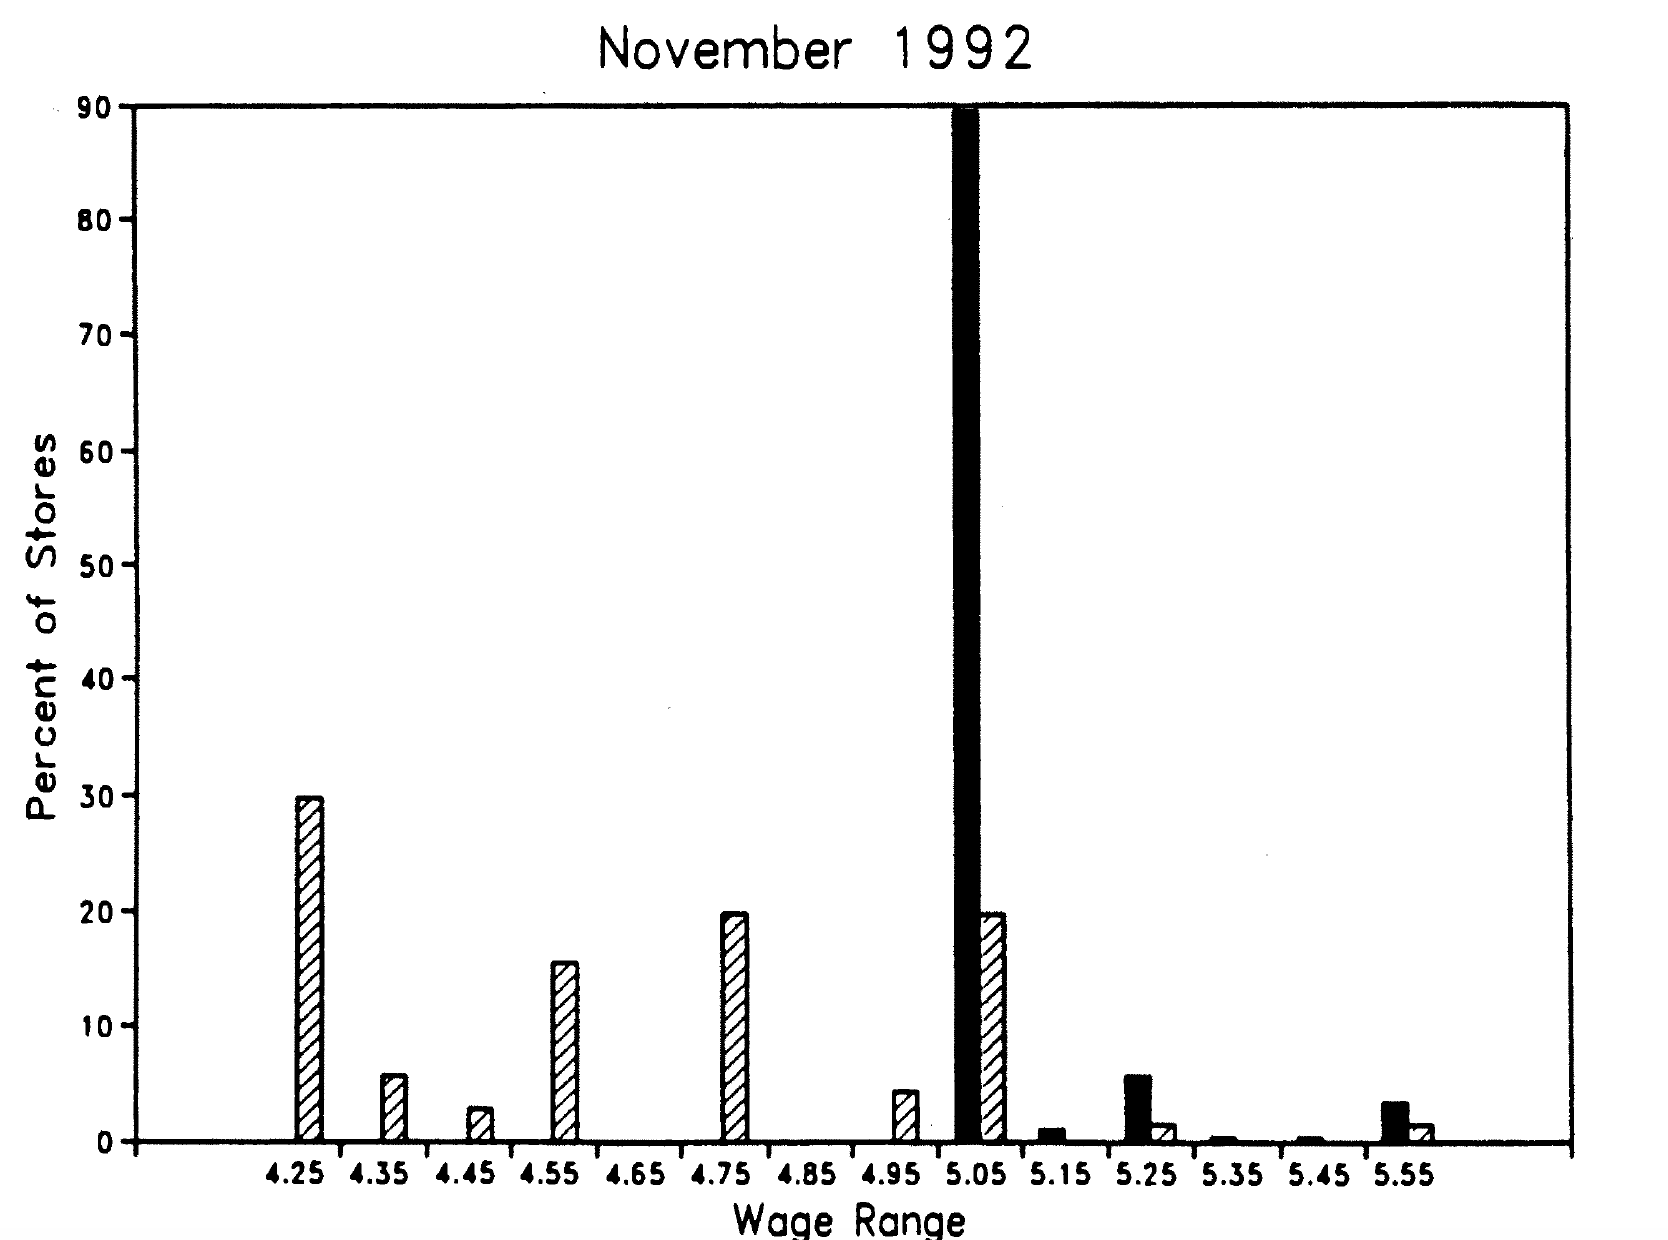
\includegraphics[scale=0.35]{nov_1992.png}
\end{center}

\end{frame}

%@@@@@@@@@@@@@@@@@@@@@@@@@@@@@@@@@@@@@@@@@@@@@@@@@
\begin{frame}
\frametitle{Recall...}

\begin{itemize}
\item If the researcher controls assignment of independent variables to observations (e.g. selection of treatment and control groups) then the data is experimental;
\bigskip
\bigskip

\item A natural experiment is a situation in which:
\begin{itemize}
\item The researcher does NOT control assignment of independent variables to observations...
\item ...but whatever does ends up creating a psuedo-randomly assigned treatment and control group anyway.
 \end{itemize}
\bigskip
\bigskip

\item So, can we extend linear regression to deal with observational data that has the characteristics of an experiment?
\end{itemize}

\end{frame}

%@@@@@@@@@@@@@@@@@@@@@@@@@@@@@@@@@@@@@@@@@@@@@@@@@
\begin{frame}
\frametitle{Difference in Differences}

\begin{itemize}
\item Say we have data in which we measure the dependent variable for four groups:
\begin{enumerate}
\item ...a `treatment' group before treatment \color{white}(fast food restaurants NJ early 1992);
\item \color{black}...a `treatment' group after treatment \color{white}(fast food restaurants NJ late 1992);
\item \color{black}...a `control' group before no treatment \color{white}(fast food restaurants PA early 1992);
\item \color{black}...a `control' group after no treatment \color{white}(fast food restaurants PA late 1992);
\end{enumerate}
\bigskip

\item[]\color{white} This data could look something like:
\end{itemize}

 \color{white}
\begin{table}[ht]
\centering
\begin{tabular}{rrrr}
 \hline
  \hline
Unit ID & Time & Group & \# of employees \\ 
  \hline
    \hline
fast food restaurant 1& 1 & NJ & 10 \\ 
fast food restaurant 1 & 2 & NJ & 11 \\ 
fast food restaurant 2 & 1 & PA & 15 \\ 
fast food restaurant 2 & 2 & PA & 12 \\ 
\vdots&\vdots&\vdots&\vdots\\
fast food restaurant 473 & 1 & NJ & 25 \\ 
fast food restaurant 473 & 2 & NJ & 32 \\ 
   \hline
      \hline
\end{tabular}
\end{table}

\end{frame}

%@@@@@@@@@@@@@@@@@@@@@@@@@@@@@@@@@@@@@@@@@@@@@@@@@
\begin{frame}
\frametitle{Difference in Differences}

\begin{itemize}
\item Say we have data in which we measure the dependent variable for four groups:
\begin{enumerate}
\item ...a `treatment' group before treatment (fast food restaurants NJ early 1992);
\item \color{black}...a `treatment' group after treatment (fast food restaurants NJ late 1992);
\item \color{black}...a `control' group before no treatment (fast food restaurants PA early 1992);
\item \color{black}...a `control' group after no treatment (fast food restaurants PA late 1992);
\end{enumerate}
\bigskip

\item[]\color{white} This data could look something like:
\end{itemize}
\color{white}
\begin{table}[ht]
\centering
\begin{tabular}{rrrr}
  \hline
  \hline
Unit ID & Time & Group & \# of employees \\ 
  \hline
    \hline
fast food restaurant 1& 1 & NJ & 10 \\ 
fast food restaurant 1 & 2 & NJ & 11 \\ 
fast food restaurant 2 & 1 & PA & 15 \\ 
fast food restaurant 2 & 2 & PA & 12 \\ 
\vdots&\vdots&\vdots&\vdots\\
fast food restaurant 473 & 1 & NJ & 25 \\ 
fast food restaurant 473 & 2 & NJ & 32 \\ 
   \hline
      \hline
\end{tabular}
\end{table}

\end{frame}

%@@@@@@@@@@@@@@@@@@@@@@@@@@@@@@@@@@@@@@@@@@@@@@@@@
\begin{frame}
\frametitle{Difference in Differences}

\begin{itemize}
\item Say we have data in which we measure the dependent variable for four groups:
\begin{enumerate}
\item ...a `treatment' group before treatment (fast food restaurants NJ early 1992);
\item \color{black}...a `treatment' group after treatment (fast food restaurants NJ late 1992);
\item \color{black}...a `control' group before no treatment (fast food restaurants PA early 1992);
\item \color{black}...a `control' group after no treatment (fast food restaurants PA late 1992);
\end{enumerate}
\bigskip

\item This data could look something like:
\end{itemize}

\begin{table}[ht]
\centering
\begin{tabular}{rlrr}
  \hline
  \hline
Unit ID & $T$ (time) & $G$ (state) & $y$ (\# of employees) \\ 
  \hline
    \hline
fast food restaurant 1& 0 (early 1992) & 1 (NJ) & 10 \\ 
fast food restaurant 1 & 1 (late 1992) & 1 (NJ) & 11 \\ 
fast food restaurant 2 & 0 (early 1992) & 0 (PA) & 15 \\ 
fast food restaurant 2 & 1 (late 1992) & 0 (PA) & 12 \\ 
\vdots&\vdots&\vdots&\vdots\\
fast food restaurant 473 & 0 (early 1992) & 1 (NJ) & 25 \\ 
fast food restaurant 473 & 1 (late 1992) & 1 (NJ) & 32 \\ 
   \hline
      \hline
\end{tabular}
\end{table}

\end{frame}

%@@@@@@@@@@@@@@@@@@@@@@@@@@@@@@@@@@@@@@@@@@@@@@@@@
\begin{frame}
\frametitle{Difference in Differences}

\begin{itemize}
\item Let's run a simple linear regression to analyze this data:\huge
\begin{align*}
y = \beta_0 + \beta_1T + \beta_2G + \beta_{12}(TG) + \varepsilon
\end{align*}
\bigskip

\normalsize
\item As usual, in this linear regression equation:
\begin{itemize}
\item $y$ is the dependent variable -- it comes from data;
\item $T$ is an indicator that is a $1$ for after treatment and $0$ for before treatment;
\item $G$ is an indicator that is $1$ for treatment group and $0$ for control group;
\item the $\beta$'s are the effects -- linear regression will learn these from data;
\item $\varepsilon$ is noise -- we don't get to observe this;
\end{itemize}

\end{itemize}

\end{frame}

%@@@@@@@@@@@@@@@@@@@@@@@@@@@@@@@@@@@@@@@@@@@@@@@@@
\begin{frame}
\frametitle{Difference in Differences}

\begin{itemize}
\item Let's run a simple linear regression to analyze this data:\huge
\begin{align*}
y = \beta_0 + \beta_1T + \beta_2G + \beta_{12}(TG) + \varepsilon
\end{align*}
\bigskip

\normalsize
\item As usual, in this linear regression equation:
\begin{itemize}
\item $y$ is the dependent variable -- it comes from data;
\item $T$ is an indicator that is a $1$ for late 1992 and $0$ for early 1992;
\item $G$ is an indicator that is $1$ for NJ and $0$ for PA;
\item the $\beta$'s are the effects -- linear regression will learn these from data;
\item $\varepsilon$ is noise -- we don't get to observe this;
\end{itemize}

\end{itemize}

\end{frame}

%@@@@@@@@@@@@@@@@@@@@@@@@@@@@@@@@@@@@@@@@@@@@@@@@@
\begin{frame}
\frametitle{Difference in Differences}

\begin{itemize}
\item Let's run a simple linear regression to analyze this data:\huge
\begin{align*}
y = \beta_0 + \beta_1T + \beta_2G + \beta_{12}(TG) + \varepsilon
\end{align*}

\normalsize
\item Check out $\beta_{12}$ -- it can be shown (though we won't) that:
\begin{align*}
\beta_{12} = (\overline{y}_{11} - \overline{y}_{01}) - (\overline{y}_{10} - \overline{y}_{00})
\end{align*}
\begin{itemize}
\item $\overline{y}_{TG} = $ average dependent variable for group $G$ at time $T$;
\item[]\color{white} $\overline{y}_{11} = $ average dependent variable for the treatment group after treatment;
\item[]\color{white} $\overline{y}_{01} = $ average dependent variable for the treatment group before treatment;
\item[]\color{white} $\overline{y}_{10} = $ average dependent variable for the control group after treatment;
\item[]\color{white} $\overline{y}_{00} = $ average dependent variable for the control group before treatment;
\end{itemize}
\end{itemize}

\end{frame}

%@@@@@@@@@@@@@@@@@@@@@@@@@@@@@@@@@@@@@@@@@@@@@@@@@
\begin{frame}
\frametitle{Difference in Differences}

\begin{itemize}
\item Let's run a simple linear regression to analyze this data:\huge
\begin{align*}
y = \beta_0 + \beta_1T + \beta_2G + \beta_{12}(TG) + \varepsilon
\end{align*}

\normalsize
\item Check out $\beta_{12}$ -- it can be shown (though we won't) that:
\begin{align*}
\beta_{12} = (\overline{y}_{11} - \overline{y}_{01}) - (\overline{y}_{10} - \overline{y}_{00})
\end{align*}
\begin{itemize}
\item $\overline{y}_{TG} = $ average dependent variable for group $G$ at time $T$;
\item $\overline{y}_{11} = $ average dependent variable for the treatment group after treatment;
\item $\overline{y}_{01} = $ average dependent variable for the treatment group before treatment;
\item $\overline{y}_{10} = $ average dependent variable for the control group after treatment;
\item $\overline{y}_{00} = $ average dependent variable for the control group before treatment;
\end{itemize}
\end{itemize}

\end{frame}

%@@@@@@@@@@@@@@@@@@@@@@@@@@@@@@@@@@@@@@@@@@@@@@@@@
\begin{frame}
\frametitle{Difference in Differences}

\begin{itemize}
\item Let's run a simple linear regression to analyze this data:\huge
\begin{align*}
y = \beta_0 + \beta_1T + \beta_2G + \beta_{12}(TG) + \varepsilon
\end{align*}

\normalsize
\item Check out $\beta_{12}$ -- it can be shown (though we won't) that:
\begin{align*}
\beta_{12} = (\overline{y}_{11} - \overline{y}_{01}) - (\overline{y}_{10} - \overline{y}_{00})
\end{align*}
\begin{itemize}
\item $\overline{y}_{TG} = $ average dependent variable for group $G$ at time $T$;
\item $\overline{y}_{11} = $ average employment for the NJ restaurants, late 92;
\item $\overline{y}_{01} = $ average employment for the NJ restaurants, early 92;
\item $\overline{y}_{10} = $ average employment for the eastern PA restaurants, late 92;
\item $\overline{y}_{00} = $ average employment for the eastern PA restaurants, early 92;
\end{itemize}
\end{itemize}

\end{frame}

%@@@@@@@@@@@@@@@@@@@@@@@@@@@@@@@@@@@@@@@@@@@@@@@@@
\begin{frame}
\frametitle{Difference in Differences}

\huge
\begin{align*}
\beta_{12} = (\overbrace{\overline{y}_{11}}^{\mbox{\normalsize NJ, late 92}} - \overbrace{\overline{y}_{01}}^{\mbox{\normalsize NJ, early 92}}) - (\overbrace{\overline{y}_{10}}^{\mbox{\normalsize PA, late 92}} - \overbrace{\overline{y}_{00}}^{\mbox{\normalsize PA, early 92}})
\end{align*}

\end{frame}

%@@@@@@@@@@@@@@@@@@@@@@@@@@@@@@@@@@@@@@@@@@@@@@@@@
\begin{frame}
\frametitle{Difference in Differences}

\huge
\begin{align*}
\beta_{12} = \underbrace{(\overbrace{\overline{y}_{11}}^{\mbox{\normalsize NJ, late 92}} - \overbrace{\overline{y}_{01}}^{\mbox{\normalsize NJ, early 92}})}_{\mbox{\normalsize Difference w/i Treatment}} - \underbrace{(\overbrace{\overline{y}_{10}}^{\mbox{\normalsize PA, late 92}} - \overbrace{\overline{y}_{00}}^{\mbox{\normalsize PA, early 92}})}_{\mbox{\normalsize Difference w/i Control}}
\end{align*}

\end{frame}

%@@@@@@@@@@@@@@@@@@@@@@@@@@@@@@@@@@@@@@@@@@@@@@@@@
\begin{frame}
\frametitle{Difference in Differences}

\huge
\begin{align*}
\beta_{12} = \underbrace{\underbrace{(\overbrace{\overline{y}_{11}}^{\mbox{\normalsize NJ, late 92}} - \overbrace{\overline{y}_{01}}^{\mbox{\normalsize NJ, early 92}})}_{\mbox{\normalsize Difference w/i Treatment}} - \underbrace{(\overbrace{\overline{y}_{10}}^{\mbox{\normalsize PA, late 92}} - \overbrace{\overline{y}_{00}}^{\mbox{\normalsize PA, early 92}})}_{\mbox{\normalsize Difference w/i Control}}}_{\mbox{Difference in Differences}}
\end{align*}

\end{frame}

%@@@@@@@@@@@@@@@@@@@@@@@@@@@@@@@@@@@@@@@@@@@@@@@@@
\begin{frame}
\frametitle{Parallel Trend Assumption}

\begin{center}
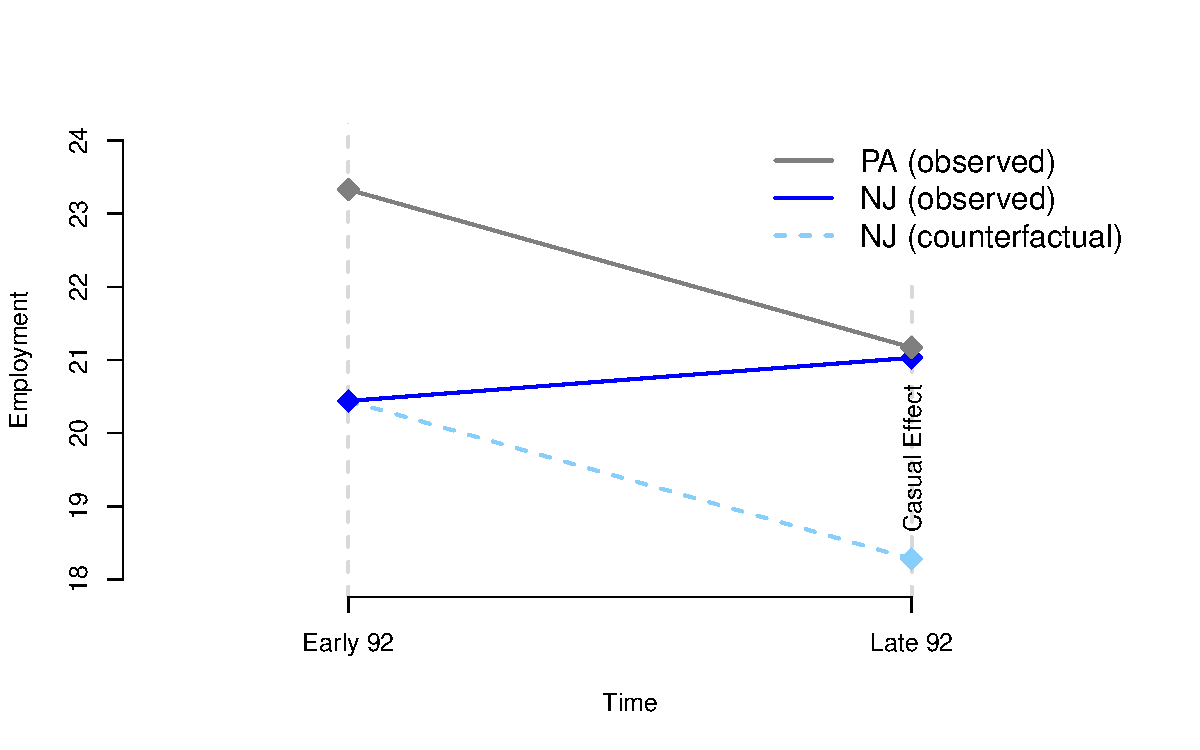
\includegraphics[scale=0.65]{common_slopes.pdf}
\end{center}

\end{frame}

%@@@@@@@@@@@@@@@@@@@@@@@@@@@@@@@@@@@@@@@@@@@@@@@@@
\begin{frame}
\frametitle{So, does increasing minimum wage decrease employment?  }

\begin{table}[ht]
\centering
\begin{tabular}{rlrr}
  \hline
  \hline
 & NJ & PA & Difference \\ 
  \hline
    \hline
Early 92 & $20.44$ & $23.33$ & $-2.89$ \\ 
Late 92 & $21.03$ & $21.17$ & $-0.14$ \\ 
Change & $0.59$ & $-2.16$ & \textbf{2.75} \\ 
   \hline
      \hline
\end{tabular}
\end{table}

\begin{align*}
\beta_{12} &= (\overline{y}_{11} - \overline{y}_{01}) - (\overline{y}_{10} - \overline{y}_{00})\\
\color{white}\beta_{12} &\color{white}= (21.03 - 20.44) - (21.17 - 23.33) = 2.75.
\end{align*}

\end{frame}

%@@@@@@@@@@@@@@@@@@@@@@@@@@@@@@@@@@@@@@@@@@@@@@@@@
\begin{frame}
\frametitle{So, does increasing minimum wage decrease employment?  Nope!}

\begin{table}[ht]
\centering
\begin{tabular}{rlrr}
  \hline
  \hline
 & NJ & PA & Difference \\ 
  \hline
    \hline
Early 92 & $20.44$ & $23.33$ & $-2.89$ \\ 
Late 92 & $21.03$ & $21.17$ & $-0.14$ \\ 
Change & $0.59$ & $-2.16$ & \textbf{2.75} \\ 
   \hline
      \hline
\end{tabular}
\end{table}

\begin{align*}
\beta_{12} &= (\overline{y}_{11} - \overline{y}_{01}) - (\overline{y}_{10} - \overline{y}_{00})\\
\beta_{12}  &= (21.03 - 20.44) - (21.17 - 23.33) = 2.75.
\end{align*}

\end{frame}

%@@@@@@@@@@@@@@@@@@@@@@@@@@@@@@@@@@@@@@@@@@@@@@@@@
\begin{frame}

\begin{center}
\Huge\textbf{Why should we care?}\\
\bigskip
\bigskip
\large Experiments are the gold standard in establishing causality and we can use linear regression to model the data they generate.\\
\end{center}

\end{frame}



\end{document}






